\section{Proposed Defense Scheme}

\begin{figure*}[h]
  \centering
    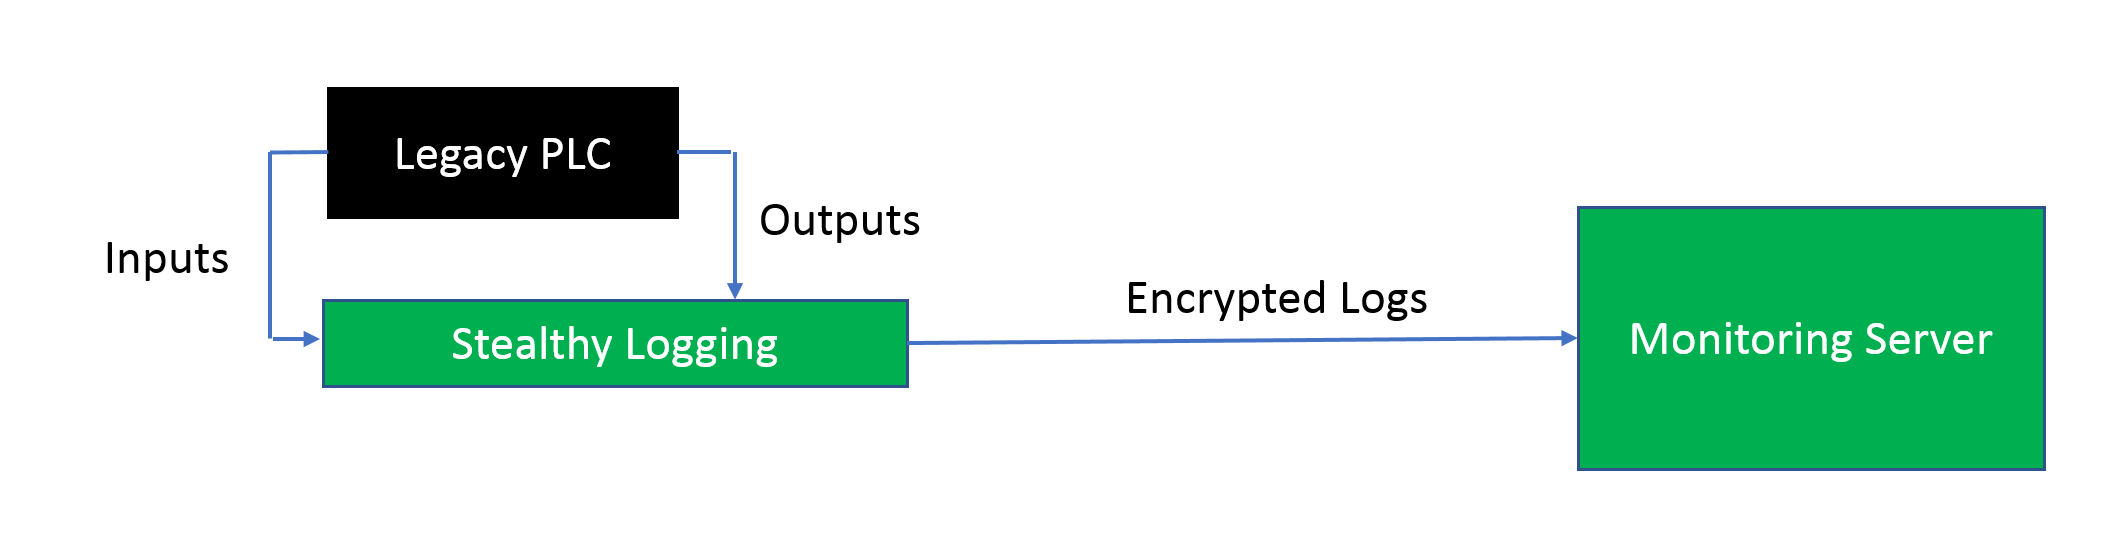
\includegraphics[width=\textwidth]{figs/legacy_system}
    \caption{Data format of one event in the log.}
    \label{fig:data_format}
\end{figure*}

\begin{figure*}[h]
  \centering
    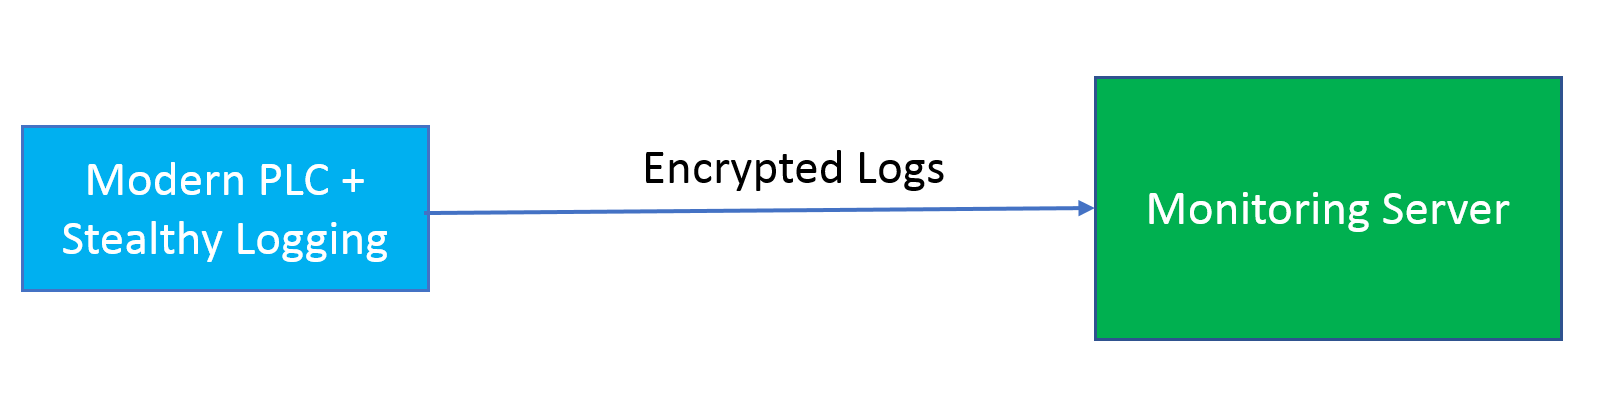
\includegraphics[width=0.8\textwidth]{figs/modern_system}
    \caption{Data format of one event in the log.}
    \label{fig:data_format}
\end{figure*}


A host-based intrusion detection (HIDS) is commonly used for monitoring specific activities and characteristics of a single device by means of software or appliance-based components known as agents. In this regard, in this project, we propose a very lightweight HIDS module on the OpenPLC framework in order to keep track of input/output operations on the device.

To locate signs of likely security related incidents, the HIDS's agent, which we call it the \emph{snapshotter} agent, essentially, takes a snapshot of the input/output values together with the current time stamps on each PLC, encrypts the log, and sends them \emph{in a stealthy secure way} to a server periodically. Forward security is achieved in the key management of the encryption key. Next key is updated to the hash of the current key after each encryption. Therefore, even the adversary compromised the device completely, meaning that the encryption key is also exposed to the adversary, he is still not able to tell from the previous encrypted logs that whether he is caught by the intrusion detection systems or not.   

Upon receiving the reports from PLCs, the server can use the received input and known PLC logic to simulate the expected output of the PLC. If the received PLC output does not match with the expected (simulated) output, then the server will conclude that this PLC has been compromised, so it should be restarted and reprogrammed by a correct logic program. Of course, for a specific application, the server can have a predefined set of acceptable input/output pairs for each device. This will reduce the computation of the server side. Besides the input/output behaviors, the integrity of the log can be checked at the server, in case that the attacker has already compromised the device.

Our defense mechanism can be summarized in security related information gathering and logging, incident identification, and taking effective actions to foil such incidents.

This solution has five features that make our proposed scheme very suitable to the intrusion detection for PLCs:

\begin{enumerate}
\item We can guarantee the integrity of the log generated by each PLCs, because we are able to verify its integrity at the server side, and we can detect any dropped package in the communication.  

\item The log is sent in a stealthy way, such that the attacker is not able to tell whether he gets detected or not. This gives more advantages to the defenders to record more behaviors of the attackers, which can be used for further investigations.  

\item This approach requires no redundant PLCs for detecting an intrusion, so it saves the cost of extra PLCs for implementing any intrusion detection schemes, e.g. comparing the outputs of two redundant PLCs. 

\item Our approach can be applied on any legacy PLCs, because we only record the inputs and outputs of each PLCs in the log. No internal states of the PLCs are required. 

\item Since the logic running on the PLCs is usually very simple, a powerful server can easily simulate a large number of PLCs in parallel. This makes our solution easily scalable to monitor a large number of PLCs.

\item In the scenario of an industrial control system, all the devices are connected using cables, so the connectivity of each PLC device is very well established. This will reduce the false positive of our system caused by the network delay. 

\end{enumerate} 


\subsection{Information Gathering}

In order to achieve the stealth logging, we suggest to use the logging mechanism in \cite{IEEEhowto:kopka}. The log has two requirements:

\begin{enumerate}
\item All the logs are encrypted, and the encryption key is updated in a forward secure key. 
\item The logs are buffered in the device itself, and is sent periodically to the server.
\end{enumerate}

The first requirement prevents the adversary, who eavesdrops the communication between the PLCs and the server, from figuring out whether the current attack is being detected or not. A forward secure key management scheme guarantees that even when the current key is compromised by the adversary, the adversary is still not able to decrypt all the encrypted logs sent before. 

The second requirement prevents the attackers from dropping all the encrypted logs that possibly record some traces of the adversary, because if the report of one device is not sent to the server on time, the server will conclude that this device has compromised by attackers.

\subsection{Incident Identification}

If any of the incidents happen, i.e., whether the log's integrity check fails, or an operation is detected as incorrect, a flag will be raised and an intrusion is indeed captured\footnote{Assuming no errors in the controller functionality itself. Note that, even if there is error in the PLC functionality, our proposed method can capture it as well with same procedure}. The server takes proper actions consequently which could be terminating the controller, revoking it from the network, or even recovering it to a previous clean/safe state.

%For the operation validation purposes, the server actually traces deviations from predefined normal profile activities/behaviors of the input/output operations. Such profile activities could be generated based on the specific applications that the PLC is being used for. (see the comments in tex file)
%what are proper server responses in case of an intrusion???
%


\subsection{Mitigation}

Once an incident has been identified, one can restart the compromised PLCs, and reprogram it to a safe/correct state/logic. If the monitoring server is not able to reset the PLC to a clean state, then a technician must be sent to physically approach the PLC and fix it. In the meanwhile, another uncompromised PLC can be deployed to replace the compromised PLC to continue the industrial process. 